%%%%%%%%%%%%%%%%%%%%%%%%%%%%%%%%%%%%%%%%%%%%%%%%%%%%%%%%%%%%%%%%%%%%%%%%%%%%%%%%%%%%%%%%%%%%%



%As explained before, the purpose is to provide a baseline to evaluate CrossSim, so it's mandatory to have a precise idea of what these approaches are and how does they work. Concerning MudaBlue and Clan, we will discuss about their rationale, showing also their original results, then we will show how we reimplemented such approaches from an high-level point of view.

%\section{MUDABlue}

%The first procedure analysed was MUDABlue, unfortunately none implentation was available on the web, so i reimplemented it from scratch. The MUDABlue method is an automatc categorizaton method of a large collecton of software systems. MUDABlue method does not only categorize sooware systems but also determines categories from the software systems collection automatigcally. MUDABlue has three major aspects: 1) it relies on no other information than the source code, 2) it determines category sets automatically, and 3) it allows a software system to be a member of multiple categories. Since we were interested only in the evaluation of the similarity we discarded the phases related to clusterization and categorization.

%\subsection{Results}
%The experimentation was conducted on a corpus of $41$ \emph{C} projects, taken form SourceForge belonging to $5$ categories.
%Developers used \emph{precision} and \emph{recall} as criteria, defined as follows:
%
%\begin{equation}
%Precision = \frac{\sum_{s\in S}\text{precision}_{soft}\text{(S)}}  {\mid S \mid}
%\end{equation}
%
%\begin{equation}
%Recall = \frac{\sum_{s\in S}\text{recall}_{soft}\text{(S)}}  {\mid S \mid}
%\end{equation}
%
%\begin{equation}
%Precision_{soft}\text{(s)} = \frac{\mid C_\text{MudaBlue}\text{(s)} \cap C_\text{Ideal}\text{(s)} \mid}  {\mid C_\text{MudaBlue}\text{(S)} \mid}
%\end{equation}
%
%\begin{equation}
%Recall_{soft}\text{(s)} = \frac{\mid C_\text{MudaBlue}\text{(s)} \cap C_\text{Ideal}\text{(s)} \mid}  {\mid C_\text{Ideal}\text{(s)} \mid}
%\end{equation}
%
%where $C_\text{MudaBlue}\text{(s)}$ is a set of categories containing software s, generated by MUDABlue, $C_\text{Ideal}\text{(s)}$ is a set of categories containing software \emph{s}, determined manually by the experimenters. In both of the criteria, the larger value,
%the better result.

%\clearpage

%%%%%%%%%%%%%%%%%%%%%%%%%%%%%%%%%%%%%%%%%%%%%%%%%%%%%%%%%%%%%%%%%%%%%%%%%%%%%%%%%%%%%%%%%%%%%

%\section{CLAN: Closely reLated ApplicatioNs}

%\subsection{Results}
%The developers used a corpus of $8310$ projects from SourceForge, for a total of $114146$ API calls. The evaluation method was similar to our, a user study with a group of 33 student of University of Illinois at Chicago with at least 6 months of java experience. Their main task was to examine the retrieved applications and to determine if they are relevant to the tasks and the source application. Each participant accomplished this step individually, assigning a confidence level, C, to the examined applications using a four-level Likert scale.

%\begin{figure}[!h]
%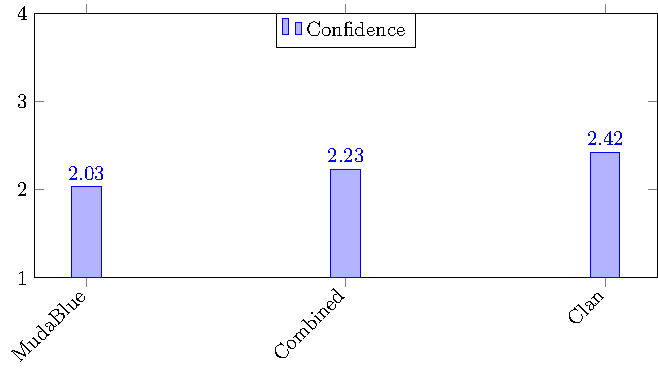
\includegraphics[width=10cm,height=15cm,keepaspectratio]{images/ConfidenceClan.pdf}
%\centering
%\caption{Confidence Comparison Original Clan}
%\label{fig:ConfidenceClan}
%\end{figure}
%
%\begin{figure}[!h]
%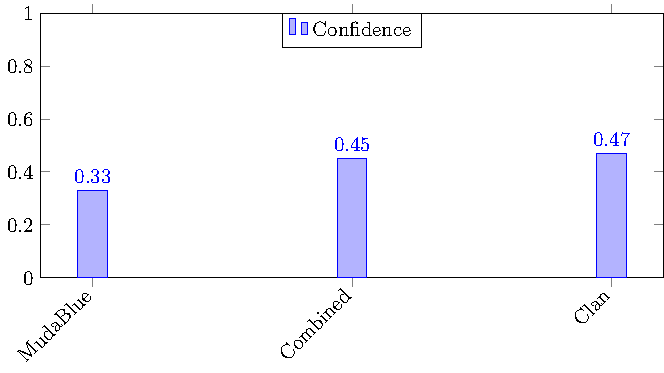
\includegraphics[width=10cm,height=15cm,keepaspectratio]{images/PrecisionClan.pdf}
%\centering
%\caption{Precision Comparison Original Clan}
%\label{fig:PrecisionClan}
%\end{figure}


%Figure \ref{fig:ConfidenceClan} and figure \ref{fig:PrecisionClan} reports the mean of the results they got from the students. As you can see the Clan approach performs better than MudaBlue. Since Similarity Matrices of MUDABlue and CLAN have the same dimensions, it is possible to construct a combined matrix whose values are the average of the values of the MUDABlue and CLAN matrix elements at the corresponding position. [nota e chiedere]

%\clearpage


%%%%%%%%%%%%%%%%%%%%%%%%%%%%%%%%%%%%%%%%%%%%%%%%%%%%%%%%%%%%%%%%%%%%%%%%%%%%%%%%%%%%%%%%%%5  

%\section{RepoPal: Exploiting Metadata to Detect Similar GitHub Repositories}\label{sec:repopal}
%
%In contrast to many previous studies that are generally based on source code \cite{10.1109/APSEC.2004.69},\cite{Liu:2006:GDS:1150402.1150522},\cite{McMillan:2012:DSS:2337223.2337267}, \textit{RepoPal}  \cite{10.1109/SANER.2017.7884605} is a high-level similarity metric and takes only repositories metadata as its input. With this approach, two GitHub repositories are considered to be similar if:
%
%\begin{itemize}
%	\item[i)] They contain similar readme files;
%	\item[ii)] They are starred by users of similar interests;
%	\item[iii)] They are starred together by the same users within a short period of time. 
%\end{itemize}
%
%Thus, the similarities between GitHub repositories are computed by using three inputs: readme file, stars and the time gap that a user stars two repositories. Considering two repositories $ r_{i} $ and $ r_{j} $, the following notations are defined: 
%
%\begin{itemize}
%	\item $ f_{i} $ and $ f_{j} $ are the readme files with $ t $ being the set of terms in the files; 
%	\item $ U(r_{i}) $ and $ U(r_{j}) $ are the set of users who starred $ r_{i} $ and $ r_{j} $, respectively; 
%	\item $ R(u_{k}) $ is the set of repositories that user $ u_{k} $ already starred.  
%\end{itemize}
%
%There are three similarity indices as follows:
%
%\paragraph{Readme-based similarity} 
%
%The similarity between two readme files is calculated as the cosine similarity between their feature vectors $\vec{f_{i}}$ and $\vec{f_{j}}$: 
%
%\begin{equation}
%sim_{f}(r_{i},r_{j})=CosineSim(\vec{f_{i}},\vec{f_{j}})
%\end{equation}
%\clearpage


%%%%%%%%%%%%%%%%%%%%%%%%%%%%%%%%%%%%%%%%%%%%%%%%%%%%%%%%%%%%%%%%%%%%%%%%%%%%%%%%%%

%\section{CrossSim}
%
%Since the purpose of this thesis is to provide implementation and data to validate CrossSim approach, is useful to explain in detail it.
%So this section we are going to present CROSSSIM (Cross Project Relationships for Computing Open Source Software Similarity), an approach that makes use of graphs for representing different kinds of relationships in the OSS ecosystem. In particular, with the adoption of the graph representation, we are able to transform the relationships among non-human artifacts, e.g. API utilizations,
%source code, interactions, and humans, e.g. developers into a mathematically computable format, i.e. one that facilitates various types of computation techniques.
%



%\section{Overview}

We select \MUDABlue, \CLAN, \RepoPal and \CrossSim as the tools to be investigated in this chapter. The rationale behind the selection of these tools for comparison is that they are well-established approaches for detecting similar OSS projects. According to \emph{Zhang et al.} \cite{10.1109/SANER.2017.7884605}, by applying the same experiment settings and evaluating on the same dataset, the authors demonstrated that \RepoPal outperforms \CLAN with respect to \emph{Confidence} and \emph{Precision}. Whereas \CLAN has a better performance than that of \MUDABlue, also with respect to \emph{Confidence} and \emph{Precision} \cite{McMillan:2012:DSS:2337223.2337267}. In addition, \RepoPal works on GitHub Java repositories containing rich metadata that is suitable for building graph by \CrossSim. Intuitively, we consider \MUDABlue, \CLAN, and \RepoPal as a good starting point for a performance comparison with \CrossSim. 

We try to exploit the original implementation of the tools. The \CrossSim source code and data are already available at the \projectName's GitHub repository \cite{CROSSSIM-DATA}. Similarly, the \RepoPal implementation can be found from one of its author's repository \cite{RepoPalImplementation}. Unfortunately, the public implementations of \MUDABlue and \CLAN are no longer available. Thus, we had to re-implement the tools by strictly following the description in the corresponding papers \cite{10.1109/APSEC.2004.69},\cite{McMillan:2012:DSS:2337223.2337267}. In the following sections, we are going to provide a description on the implementation of \MUDABlue and \CLAN.


%%%%%%%%%%%%%%%%%%%%%%%%%%%%%%%%%%%%%%%%%%%%%%%%%%%%%%%%%%%%%%%%%%%%%%%%%%%% 

\section{System Description}

%This section explains our work and what we have done. In order to do this we will use some UML diagram plus a generich high level architecture diagram.
%This image, exctracted from CrossSim documentation depicts how a similarity calculator fits inside a real project. It is clear that in order to provide a meaningful recommendation, it is mandatory to have a similarity calculator better as possible since all the functionality extending the \emph{GetProjectAlternatives} use case, rely on some similarity computation. As you can see there are 5 main components:

The use cases concerning the functionality of finding similar OSS projects are depicted in Figure~\ref{fig:UseCases}. These use cases are directly extracted from the \projectName pr\-oject document. The Component Diagram is shown in Figure~\ref{fig:Components} and there are the following components:

\begin{figure}[!h]
	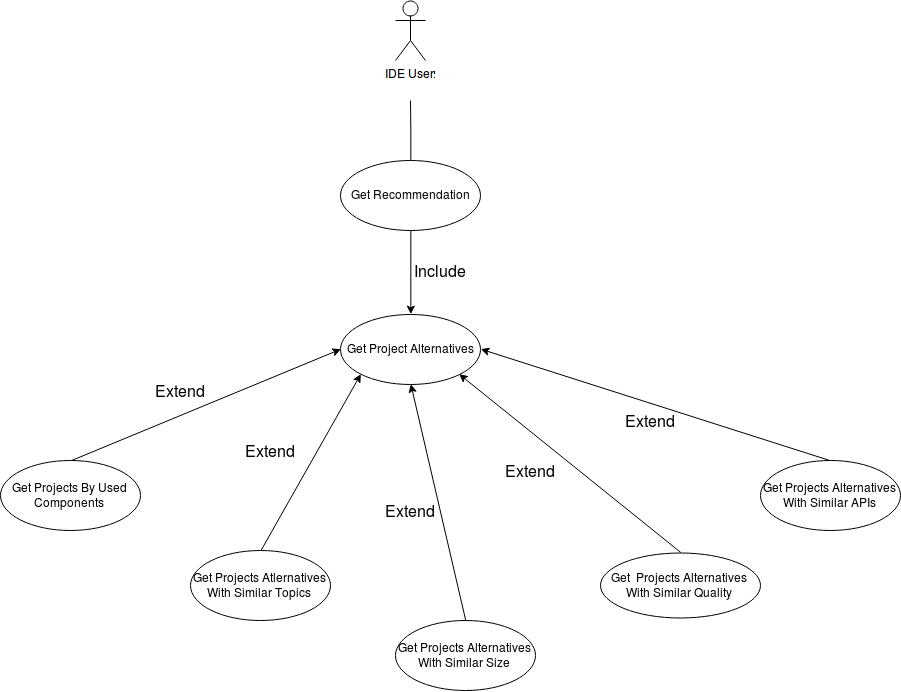
\includegraphics[width=15cm,height=20cm,keepaspectratio]{images/UseCaseDiagram.png}
	\caption{The Use Case Diagram}
	\label{fig:UseCases}
\end{figure}

%\subsection{Component Point of View}

\begin{figure}[!h]
	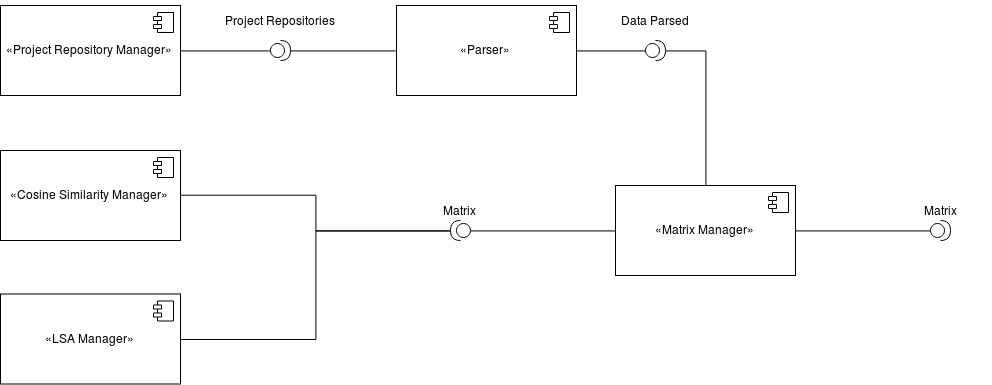
\includegraphics[width=15cm,height=20cm,keepaspectratio]{images/ComponentDiagram.png}
	\caption{Component Diagram}
	\label{fig:Components}
\end{figure}



\begin{itemize}
	\item Project Repository manager: this is the component that provides the repositories and manages the file system.
	\item Parser: this component analyzes all the \emph{.java} files in order to retrieve the keywords to create the term-document matrix. As stated before we search for the \emph{JDK} related imports and methods for \CLAN and any imports, method, variables and field variables for \MUDABlue.
	\item Matrix Manager: this is the central component, it manages the creation of the term-document matrix, and coordinates all the matrices "roaming" during the process. %For example the term-document matrix can't be analyzed as it is by the SVD component.%, it requires a rework before.
	\item LSA Manager: by this component all the operations concerning the Latent Semantic Analysis occur, from the low-rank matrix reduction to the Singular Value Decomposition.
	\item Cosine Similarity Manager: once the LSA completes its work, cosine similarity is then applied to get the final version of the matrix.
\end{itemize}


\begin{figure}[!h]
	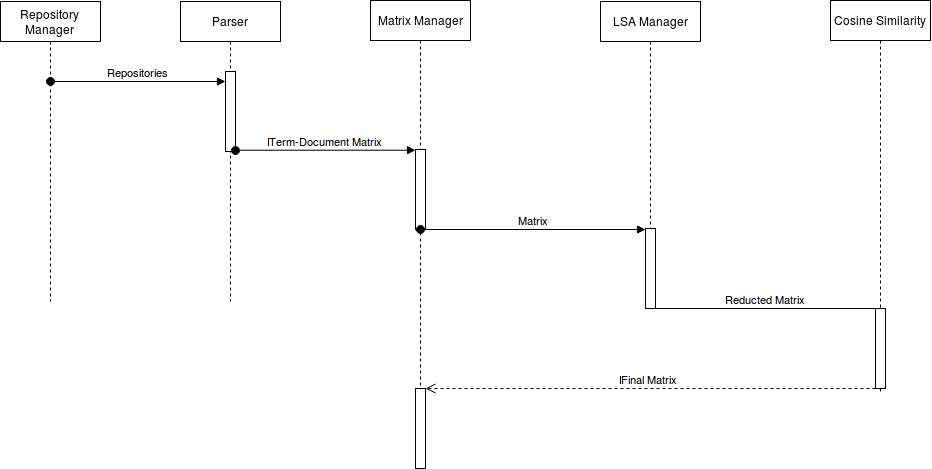
\includegraphics[width=15cm,height=20cm,keepaspectratio]{images/SequenceDiagram.png}
	\caption{Sequence Diagram}
	\label{fig:Sequence}
\end{figure}

Figure~\ref{fig:Sequence} depicts the sequence diagram. When the process starts, the Project Repository Manager analyzes its file system in order to provide all the repositories to be analyzed. It also checks if the parsing has already occurred, this is due to the extremely high consumption of memory, thus the phases have been split in two moments. Once the repositories to be analyzed are known, the process can start. As already explained before, for \MUDABlue and \CLAN the terms are different, however the same library  \emph{Java Parser} is used in both cases. The outcome is a term-document matrix which is processed by the Latent Semantic Analysis manager. The \emph{commons math} component is used to decompose the matrix. Afterwards, the LSA matrix is obtained by multiplying the matrices. At this stage, it is necessary to take the matrix and then apply the cosine similarity. For each vector of the matrix, we calculate the cosine with all the others vectors. In this way, we get a final matrix of $580 \times 580$ which can be fed as input for further computations.

\section{System Structure}

\begin{figure}[!h]
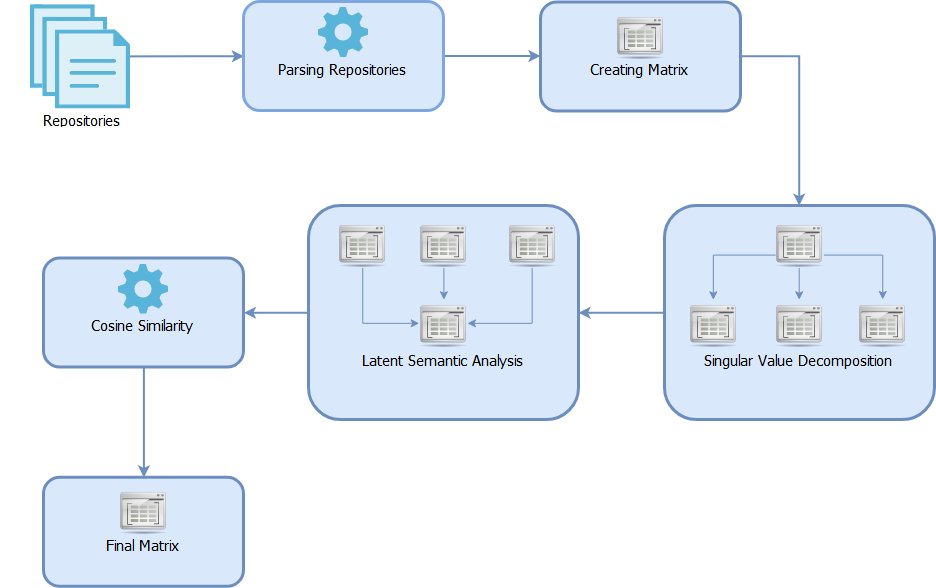
\includegraphics[width=15cm,height=20cm,keepaspectratio]{images/Architecture.png}
\caption{System Structure}
\label{fig:SystemStructure}
\end{figure}

Figure~\ref{fig:Sequence} shows the general architecture of the implemented systems. The process consists of the following steps. %as you can see the systems share the same architecture with some differences that will be discussed later.

\begin{itemize}
 \item Retrieving the dataset, in this case a folder with all $580$ repositories.
 \item All the \code{.java} files are parsed.
 \item Each repository is represented as a vector that contains all the frequencies.% and then added in a matrix. 
 \item The SVD procedure is applied to decompose the matrix into $3$ matrices.
 \item The matrices are multiplied back to realize the LSA procedure.
 \item Similarity between every vector is computed against all the remaining vectors.%For each vector, we count the cosine similarity with all the others.
 \item Eventually, the final similarity matrix is created.%, where any repositories is compared to all the others.
\end{itemize} 

%\section{System Details}

%Figure~\ref{fig:SystemDetails} depicts 
%
%\begin{figure}[!h]
%	\centering
%	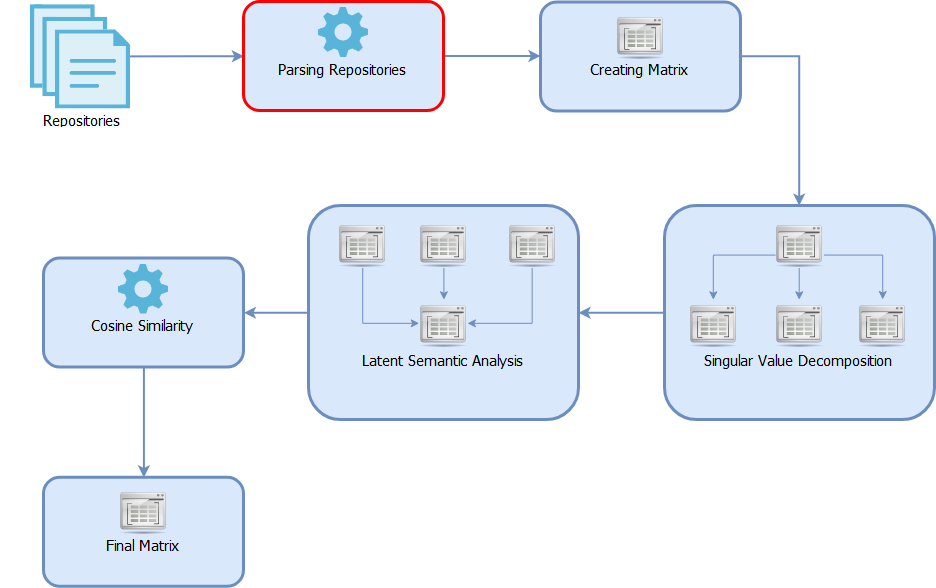
\includegraphics[width=0.8\textwidth]{images/Architecture1.png}
%	\caption{Parsing}
%	\label{fig:SystemDetails}
%\end{figure}

The parsing step is conducted on all \code{.java} files of the $580$ repositories using Java Parser. The main components of the files (import and method invocation for \CLAN, import, method declaration, variables and field variables for \MUDABlue). For each repository we created a relative \code{.txt} file containing the frequencies. For \CLAN such terms are filtered by searching only the terms belonging to the Java JDK. All these terms are merged to create another file, called \code{mainlist.txt} which is used to avoid reps. The idea is to parse the files and compare with the \code{mainlist.txt} to add new terms, and then count, for each term how many times it appears inside the files. The final result is a vector of numbers.

%\begin{figure}[!h]
%	\centering
%	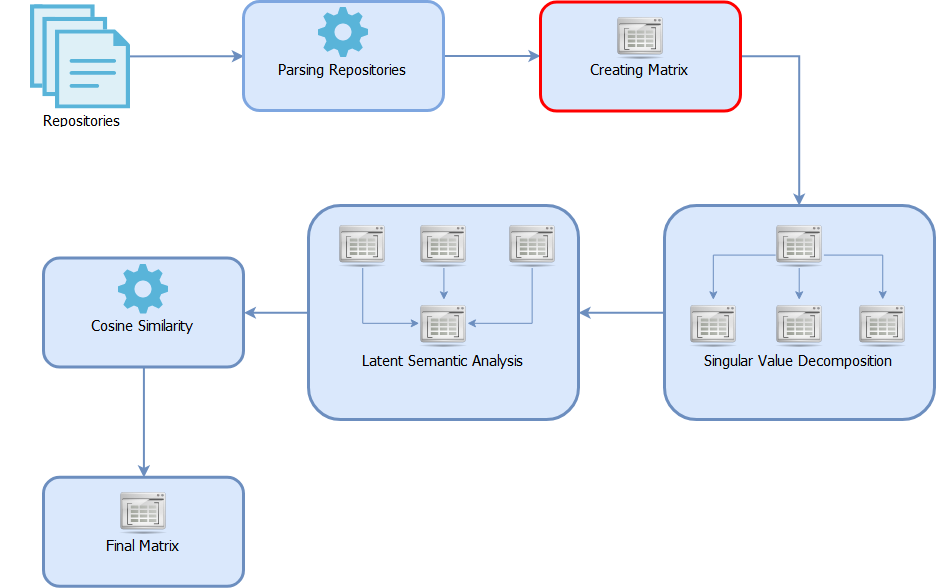
\includegraphics[width=0.8\textwidth]{images/Architecture2.png}
%	\caption{Matrix Creation}
%\end{figure}

Matrix Creation: Once all the repositories are analyzed, the term-document matrix can be created using the \emph{apache commons math3} library, in particular the following components:

\begin{itemize}
\item ArrayRealVector.
\item RealMatrix.
\item RealVector.
\end{itemize}

Each file contains only its own terms, so the idea is, once the parsing process is done, to count how many terms we have and then, to add fill the missing terms with zeros. For example, considering a set of $3$ documents \emph{A,B,C} for $10$ different terms, document contains $4$ terms, this means that the other 6 terms are missing, so they are represented as $0$.

%\begin{figure}[!h]
%	\centering
%	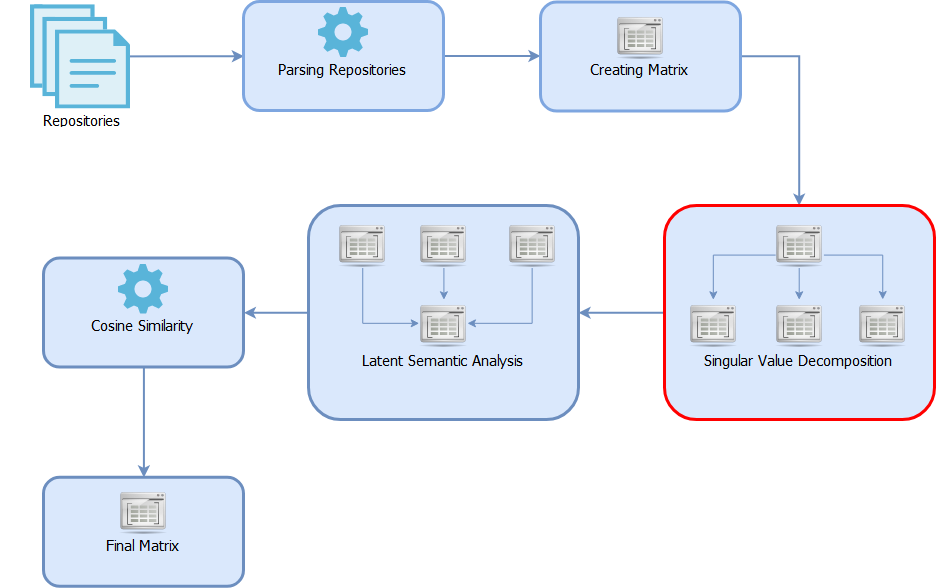
\includegraphics[width=0.8\textwidth]{images/Architecture3.png}
%	\caption{Singular Value Decomposition}
%\end{figure}

SVD: As stated before the SVD operation is used to decompose the main matrix into $3$ different matrices using \emph{math3 linear SingularValueDecomposition}. So we invoke the methods and pass as parameter the term-document matrix. %As you can see this operation was already available in the library, so we just retrieved the results of the operation.


%\begin{equation}
%A_{mn}=U_{mm}S_{mn}V_{mn}^{T}
%\end{equation}
%
%in which
%
%\begin{itemize}
%	\item $U_{mm}$: Orthogonal matrix.
%	\item $S_{mn}$: Diagonal matrix.
%	\item $V_{mn}^{T}$: The transpose of an orthogonal matrix.
%	\item $X$: Low Rank matrix.
%\end{itemize}

%\begin{figure}[!h]
%	\centering
%	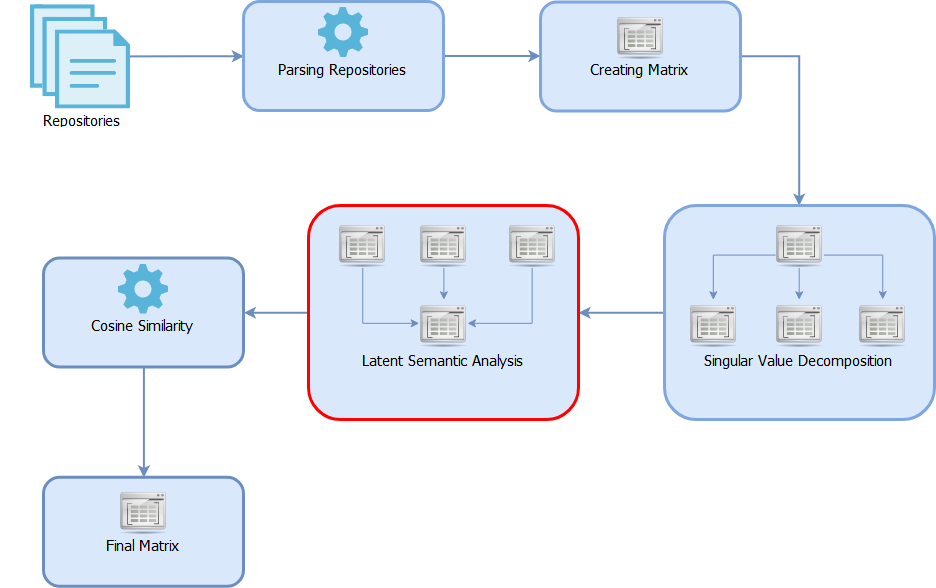
\includegraphics[width=0.8\textwidth]{images/Architecture4.png}
%	\caption{Latent Semantic Analysis}
%\end{figure}


LSA: Since there is no implementation of Latent Semantic Analysis available, we had to re-implement it from scratch. Among others, the most important issue is to identify a suitable value \emph{k} for the reduced rank. We empirically selected a value of total $\frac{repository}{2}$. The computation complexity is a key issue since a total of memory needed for a matrix is as follows:

\begin{equation}
Memory\,in\,gigabytes\,=\,\frac{(columns*rows*8)}{(1024*1024*1024)}
\end{equation}


For \MUDABlue, we got $700,000$ distinct terms for a total of 3GB of dedicated memory just for storing the matrix, without considering any kind of operations. This is due to the fact that \MUDABlue takes many different terms from a file into consideration. In contrast, \CLAN focuses only on the import and method that belong to the \emph{JDK} and this helps greatly reduce the number of distinct terms. A possible solution is to increase the available memory for Eclipse up to 8GB. Even then, many crashes can be seen. Thus, we need to perform some refactoring in the code in order to save memory, e.g. by deleting unused data structure, or using more light structures, etc.


%\begin{figure}[!h]
%	\centering
%	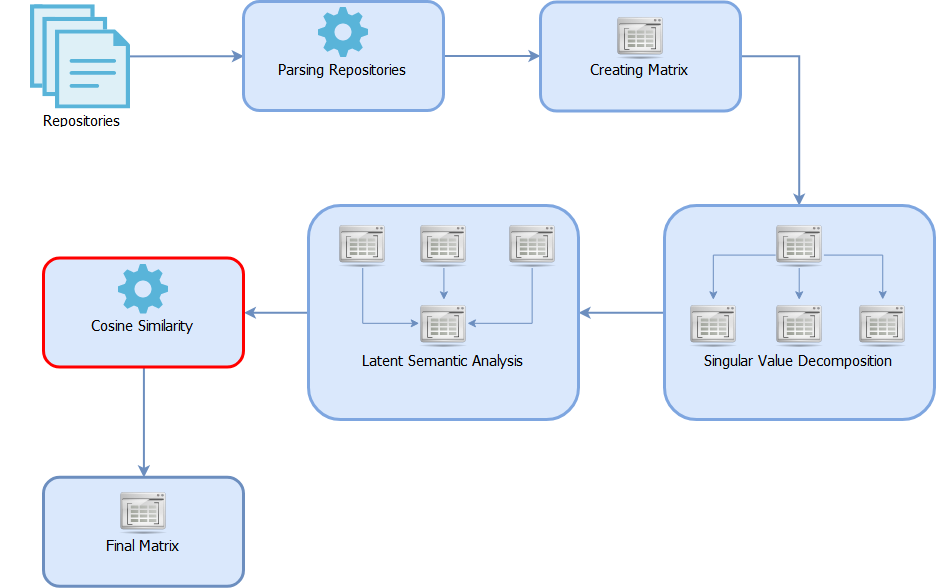
\includegraphics[width=0.8\textwidth]{images/Architecture5.png}
%	\caption{Cosine Smilarity}
%\end{figure}

By cosine similarity we mean a measure of similarity between two non-zero vectors of an inner product space that measures the cosine of the angle between them. As for \emph{LSA}, so the method takes as input two vectors and performs the operation. Since in the final matrix we have the similarity between \emph{repo1 - repo2} and \emph{repo2 - repo1}, the computation is done only for one pair in order to cut half of the calculation.

%\begin{figure}[!h]
%	\centering
%	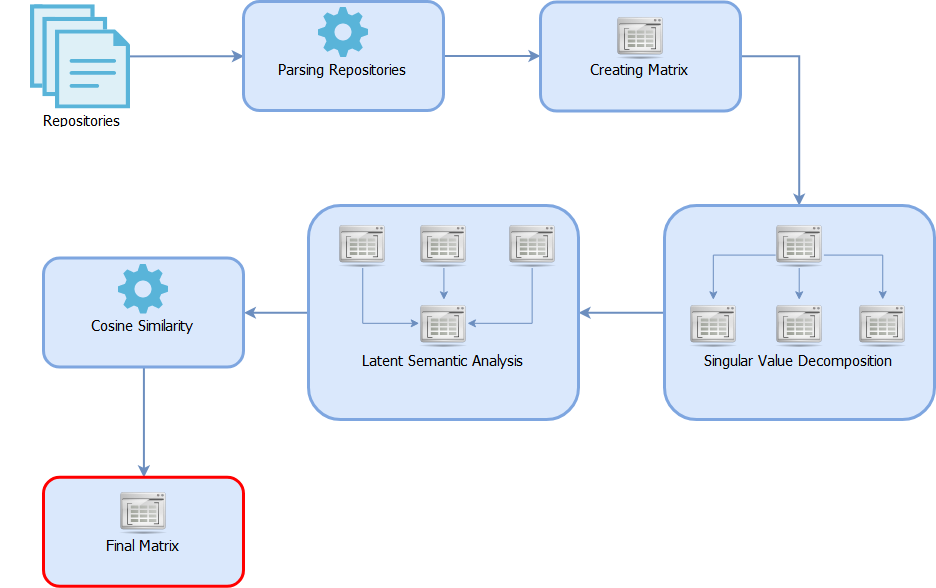
\includegraphics[width=0.8\textwidth]{images/Architecture6.png}
%	\caption{Final Matrix}
%\end{figure}

At this stage the matrix is of $580 \times 580$ in size, and with values ranging between \emph{0.0} and \emph{1.0}. This matrix is actually a collection of vectors, representing the similarity of a project with all the other projects.
The final matrix $\| M \|$ is square matrix whose rows and columns represent projects. %In particular, for any two project $P_i$ and $P_j$, each element of the matrix $M_{i,j}$ represents the similarity score defined as follows: \\

\begin{equation}
  M_{i,j}=\begin{cases}
    0\leq M \leq 1 \; \; \; \text{if i} \neq \text{j}\\
    \\
    1 \; \; \; \text{if i = j}.
  \end{cases}
\end{equation}\\

%There is one more step for \CLAN, since the approach consider the matrices separately, that is, at this stage we have two different matrices, one for the imports and one for the methods. So we have to sum up both in order to get the final one.

%%%%%%%%%%%%%%%%%%%%%%%%%%%%%%%%%%%%%%%%%%%%%%%%%%%%%%%%%%%%%%%%%%%%%%%%%%%%%%%%%%%%%%%%%%%
%\newpage

\section{Tools and Libraries}

The implementations have been conducted using Eclipse IDE Oxygen .2 and the following libraries:

\begin{itemize}
\item \textbf{org.eclipse.jdt.core 3.10.0}: this is the core part of Eclipse's Java development tools. It contains the non-UI support for compiling and working with Java code, including the following tools:
	\begin{itemize}
	\item An incremental or batch Java compiler that can run standalone or as part of the Eclipse IDE.
	\item Java source and class file indexer and search infrastructure.
	\item A Java source code formatter.
	\item APIs for code assist, access to the AST and structured manipulation of Java source.
	\end{itemize}
\item \textbf{eclipse-astparser 8.1}: this is used to analyze the AST at runtime on Eclipse.
\item \textbf{commons-math3 3.6.1}: it is a library of lightweight, self-contained mathematics and statistics components addressing the most common problems not available in the Java programming language or Commons Lang. In particular it is used to compute the SVD, singular value decomposition.
\item \textbf{commons-text 1.2}: Apache Commons Text is a library focused on algorithms working on strings. 
\item \textbf{javaparser-core 3.5.14}: This is a library for parsing \code{.java} files.
\item \textbf{ejml-0.33}: Efficient Java Matrix Library (EJML) is a linear algebra library for manipulating real/complex/dense/sparse matrices. The design goals are: 1) to be as computationally and memory efficient as possible for both small and large matrices, and 2) to be accessible to both novices and experts. These goals are accomplished by dynamically selecting the best algorithms to use at runtime, clean API, and multiple interfaces.
\end{itemize}

%%%%%%%%%%%%%%%%%%%%%%%%%%%%%%%%%%%%%%%%%%%%%%%%%%%%%%%%%%  